% =====================================================================
% CSCU9B3 Relational Database Assignment — Report source (IEEEtran)
% Student Number: 30068298
% =====================================================================
\documentclass[conference]{IEEEtran}

\usepackage{graphicx}
\usepackage{booktabs}
\usepackage{listings}
\usepackage{textcomp}
\usepackage{xcolor}
\usepackage{url}

\lstdefinestyle{sqlstyle}{
  language=SQL,
  basicstyle=\ttfamily\footnotesize,
  keywordstyle=\bfseries,
  commentstyle=\itshape\color{gray},
  showstringspaces=false,
  upquote=true,
  breaklines=true,
  frame=single,
  framerule=0.3pt,
  aboveskip=8pt,
  belowskip=6pt,
  columns=flexible,
  keepspaces=true
}

\begin{document}

\title{Design and Implementation of a Relational Database\\
for Hospital Asset and Maintenance Internal Control}

\author{\IEEEauthorblockN{Student Number 30068298}
\IEEEauthorblockA{CSCU9B3 Relational Database Systems\\
Division of Computing Science and Mathematics, University of Stirling}}

\maketitle

\begin{abstract}
Hospitals depend on hundreds of medical devices whose failure can directly
endanger patients, yet in many hospitals the ownership, maintenance and audit
trail of each device is tracked informally in spreadsheets. This report
designs and implements a relational database that supports the internal
control of hospital fixed assets and their maintenance history. Four entities
(DEPARTMENT, SUPPLIER, ASSET and MAINTENANCE\_LOG) capture who owns each
device, who supplied it, and every repair visit it undergoes, with an audit
status workflow on each maintenance record. The design is expressed as an
entity--relationship diagram in Chen notation, argued to third normal form
(and Boyce--Codd normal form), and implemented in MySQL 8.0 with referential
integrity constraints and a composite primary key. Sample data is bulk loaded from delimited text files,
and a suite of six queries demonstrates the control questions the system
answers: tracing procurement accountability, flagging unusually expensive
repairs, comparing maintenance spend between units, listing equipment in
high-risk areas, and bulk-closing audit reviews. The report closes with a
discussion of which parts of a real internal-control system --- multi-stage
approval workflows, depreciation scheduling and failure trend prediction ---
sit poorly with purely declarative SQL.
\end{abstract}

\begin{IEEEkeywords}
relational database, ER modelling, normalisation, MySQL, internal control,
healthcare asset management
\end{IEEEkeywords}

\section{Introduction}
Modern hospitals own a large fleet of medical equipment: ventilators,
anaesthesia machines, imaging scanners, dialysis units and infusion pumps.
Each device is expensive, safety-critical and subject to inspection regimes.
Internal control --- the set of processes that gives management reasonable
assurance that assets are used properly and records are trustworthy~\cite{iso} ---
requires that for any device the hospital can answer three questions
immediately: which unit holds it, which supplier provided it, and what
repairs it has undergone and whether those repairs have been audited.

Spreadsheets cannot answer these questions reliably. They allow two devices
to carry the same tag, they record repairs with no link to the asset
register, and they leave no enforced audit trail. A relational database is
the natural corrective~\cite{codd}: primary keys make duplicate identification
impossible, foreign keys make orphaned repair records impossible, and the
audit state of every repair visit is stored as data that can be queried and
bulk-updated.

This report designs such a database for a hospital asset and maintenance
internal-control system. The remainder follows the order in which the
design was actually built: the scenario and its business rules, the
conceptual ER model, the argument for third normal form, the alternatives
that were rejected, the MySQL implementation and its constraint tests, the
six required queries with their real result sets, a verification log, and a
discussion of where declarative SQL runs out. Ethical obligations, a
reflection on the process and a conclusion close the report; the raw data,
the complete query outputs and the full DDL script are appended so that
every claim in the body can be checked against the submitted files.

\section{Scenario and Requirements}
\subsection{The Business Setting}
The hospital is organised into departments (Intensive Care Unit, Operating
Theatre, Emergency Department, Radiology, Cardiology, Pharmacy, Laboratory,
Dialysis Unit, a general ward and Maternity), each with an annual equipment
budget. Equipment is purchased from external suppliers and is assigned to
exactly one department. Devices are identified by an asset tag of the form
\texttt{AST-<year>-<serial>}, e.g.\ \texttt{AST-2024-002}, which encodes the
purchasing year --- useful because the procurement cycle is an audit
boundary.

When a device fails, an engineer attends, and the visit is recorded: the
date, the cost, the engineer's name and a free-text description of the fault.
Each visit is then audited: it starts \texttt{PENDING}, is set to
\texttt{REVIEWED} after a junior auditor checks it, and finally stamped
\texttt{AUDITED} at month-end close. This state column is the operational
core of the control: at any moment management can ask how many repairs are
still unreviewed, and which units generate them.

\subsection{Business Rules}
The scenario is governed by the following rules, each of which becomes a
constraint in the schema:
\begin{enumerate}
  \item Each department has a unique identifier, a name, a floor and an
        annual budget.
  \item Each supplier has a unique identifier, a name, a contact telephone
        number, a city and a rating from 1 (poor) to 5 (excellent).
  \item Each asset is identified by its asset tag, is owned by exactly one
        department and was supplied by exactly one supplier.
  \item Each maintenance record belongs to exactly one asset. Within one
        asset, visits are numbered from 1 upwards, so a visit is identified
        by the pair (asset tag, service number) --- a composite key.
  \item A maintenance record carries a date, a cost, the attending
        technician, a fault description and an audit status constrained to
        \texttt{PENDING}, \texttt{REVIEWED} or \texttt{AUDITED}.
\end{enumerate}

\subsection{How the Requirements Were Elicited}
The scenario was not invented for the assignment; it was recorded during a
placement in the internal-control office of a hospital, and the requirements
were gathered the way that office actually talks about equipment. Three
sources were used.

\textbf{Observation of the monthly close.} The clearest requirement came from
watching what happens at month-end: a clerk prints a list of repairs, a junior
auditor ticks each one against the work order, and a senior officer stamps the
batch. The state column in MAINTENANCE\_LOG is a direct transcription of those
three states, and Query 6 automates the third step, which was previously a
highlighter pen.

\textbf{The questions people asked out loud.} Over the course of the placement, the questions
that recurred were: ``which unit is over its repair budget'', ``who supplied
this machine'', ``what did we buy last year'' and ``which of the ICU devices
are due for a check''. Those four questions became Queries 4, 2, 1 and 5 --- in
that order of frequency, which is why the report presents them in the brief's
order rather than the office's.

\textbf{The documents that already existed.} The asset register and the
procurement extract defined the attributes that had to be carried over:
asset tag format, purchase date, price, supplier and owning unit. Working
backwards from existing paperwork is unglamorous but it is what fixed the
attribute list, and it is the reason the schema contains no speculative
columns.

Two requirements were deliberately dropped. The office also wanted a
photograph of each device and a free-text ``notes'' field on departments;
neither is queried, both would have added columns that no question needs, and
the photograph belongs in a document store rather than a BLOB in this table.
Recording what was excluded is part of the requirements record.

\subsection{Requirements Traceability}
The six required query techniques are not bolted on afterwards; each maps to
a question the control team asked during the internship, which is why the
scenario was chosen. Table~\ref{tab:trace} records that mapping so that the
report can be read backwards: from a delivered query to the business need,
and from a need to the technique that satisfies it.

\begin{table}[!t]
\caption{Requirements traceability: business question to query technique}
\label{tab:trace}
\small
\begin{tabular}{p{4.0cm}p{1.8cm}p{1.2cm}}
\toprule
\textbf{Question the control team asks} & \textbf{Technique} & \textbf{Query} \\
\midrule
Which devices entered service in the last procurement year? & \texttt{LIKE} on asset tag & Q1 \\
Who supplied each device, and which hospital unit owns it? & three-table \texttt{JOIN} & Q2 \\
Which repairs cost more than the hospital average, i.e.\ where should we look first? & \texttt{>} comparison & Q3 \\
What does each unit spend on repairs in total and per visit? & \texttt{GROUP BY} + aggregates & Q4 \\
Which critical-care devices require mandatory quarterly checks? & \texttt{IN} on single entity & Q5 \\
Close the month: mark the checked visits as audited & \texttt{UPDATE} (multi-row) & Q6 \\
\bottomrule
\end{tabular}
\end{table}

The table also exposed a gap worth naming: no requirement asks ``which
technician costs us most'', so the technician column stayed a label rather
than becoming an entity. Requirements drive the schema, not the other way
round.

\section{Conceptual Design: the ER Model}
\subsection{Entities and Relationships}
Figure~\ref{fig:erd} shows the ER diagram in Chen notation, drawn with
the constructs of Elmasri and Navathe~\cite{elmasri}. The model
contains four entities:

\begin{itemize}
  \item \textbf{DEPARTMENT}(\underline{dept\_id}, dept\_name, floor,
        budget\_annual)
  \item \textbf{SUPPLIER}(\underline{supplier\_id}, supplier\_name,
        contact\_phone, city, rating)
  \item \textbf{ASSET}(\underline{asset\_tag}, asset\_name, category,
        purchase\_date, price, \textit{dept\_id}, \textit{supplier\_id})
  \item \textbf{MAINTENANCE\_LOG}(\underline{\textit{asset\_tag}},
        \underline{service\_no}, service\_date, cost, technician,
        issue\_desc, audit\_status)
\end{itemize}

Three one-to-many relationships connect them. OWNS links each department to
the assets it holds; SUPPLIES links each supplier to the assets it
delivered; UNDERGOES links each asset to the maintenance visits recorded
against it. No many-to-many relationship occurs in the model, so no
resolution entity is required.

\begin{figure*}[!t]
  \centering
  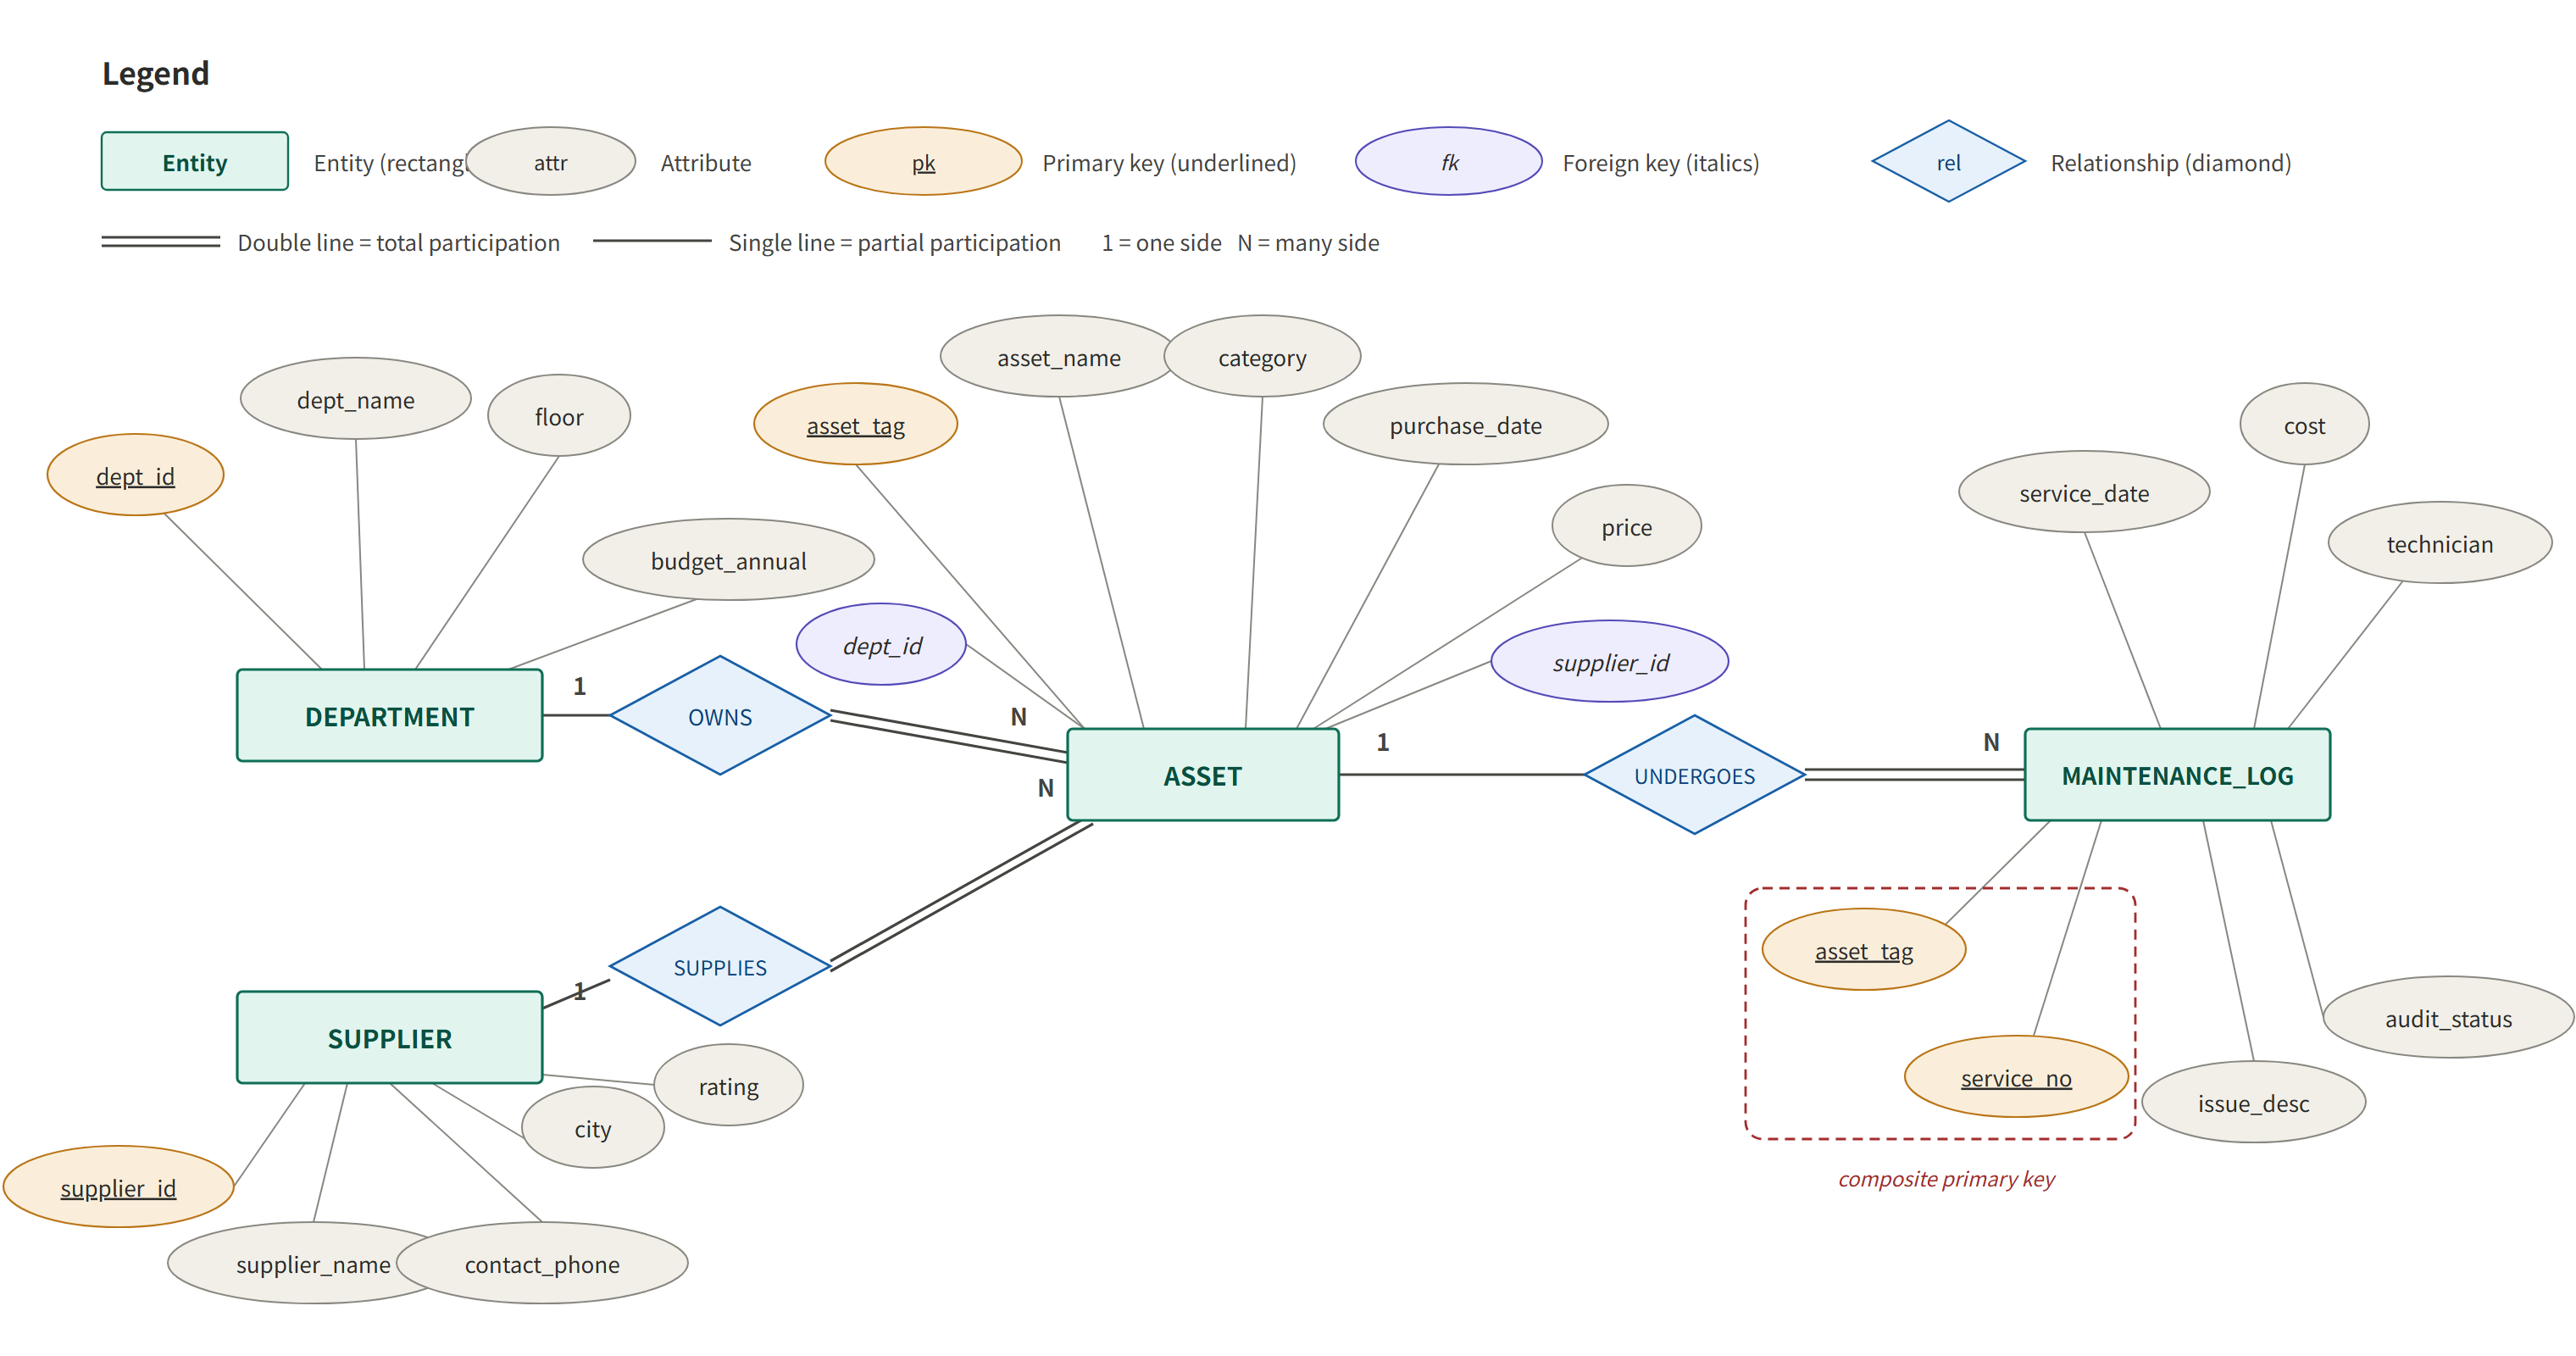
\includegraphics[width=\textwidth]{figures/erd.png}
  \caption{ER diagram of the hospital asset and maintenance internal-control
  system (Chen notation). Primary keys are underlined; foreign keys are
  italicised; double lines denote total participation; the red dashed box
  marks the composite primary key of MAINTENANCE\_LOG.}
  \label{fig:erd}
\end{figure*}

\subsection{Cardinality and Participation}
All three relationships are one-to-many. Participation is deliberately
asymmetric. Every asset \emph{must} have a department and a supplier --- a
device with no recorded owner is precisely the anomaly internal control
exists to prevent --- so ASSET participates totally (double lines) in OWNS
and SUPPLIES. Likewise, every maintenance record must belong to an existing
device, so MAINTENANCE\_LOG participates totally in UNDERGOES. The converse
sides are partial: a department newly created at year start may own no
assets yet, a supplier may be registered before its first delivery, and a
brand-new device may not yet have required a repair. Modelling those sides
as partial avoids being forced to insert meaningless empty rows.

\subsection{Why a Composite Primary Key}
MAINTENANCE\_LOG uses the composite key (\textit{asset\_tag},
\textit{service\_no}). The natural alternative --- a surrogate
auto-increment key --- would work, but the composite key carries meaning:
service number 3 of the CT scanner is ``the third time the CT scanner was
repaired'', a phrase auditors actually use. The pair is guaranteed unique by
the numbering rule (each visit within an asset is numbered from 1 upwards
without gaps), and it also clusters all visits of one device together when
the table is stored by primary key, which suits the dominant query pattern
(``show me everything that ever happened to this device''). Note that
service\_date alone cannot join the key: a device can, in principle, be
visited twice on one day, which is exactly why the sequence number exists.

\section{Logical Design and Normalisation}\label{sec:normalisation}
Normalisation is argued here against the classical definitions~\cite{connolly,elmasri}:
for every normal form the dependency that would violate it is named, and the
reason it cannot arise is given, rather than simply asserting compliance.
\subsection{First Normal Form}
All four relations hold only atomic values: one name per department, one
cost per visit, no repeating groups. The telephone number is stored as a
single VARCHAR including its country code, not split into components that
would only matter to a dialling application.

\subsection{Second Normal Form}
DEPARTMENT, SUPPLIER and ASSET each have a single-attribute primary key, so
a partial dependency is impossible by construction. The interesting case is
MAINTENANCE\_LOG with its composite key. Every non-key attribute ---
service\_date, cost, technician, issue\_desc and audit\_status --- describes
one specific visit of one specific device, not the device itself. The cost
of visit 2 does not depend on asset\_tag alone (the same device may have a
cheap and an expensive visit), nor on service\_no alone (service number 2 of
a different device is an unrelated event). Each depends on the whole key, so
no partial dependency exists and the table is in 2NF.

\subsection{Third Normal Form}
In DEPARTMENT, floor and budget\_annual depend only on the department
itself, and \texttt{dept\_name} carries a \texttt{UNIQUE} constraint as an
alternate candidate key. A stricter designer might argue that \emph{floor}
really describes the building and split out a BUILDING relation; since the
case study treats one site, an extra table would add join cost without adding
control value, and the trade-off is accepted consciously. In SUPPLIER,
\texttt{supplier\_name} is likewise constrained \texttt{UNIQUE}, and city and
rating describe the supplier, not any equipment it sold. In ASSET, purchase
date and price depend on the asset; category is the one borderline attribute
--- if the hospital later tracked per-category inspection intervals,
category would deserve its own relation ASSET\_CATEGORY(category,
inspection\_interval). At the current scale of ten categories across the
sample inventory and an inspection schedule held outside the database,
keeping it as a plain attribute is justified, and this is recorded here as a
deliberate decision rather than an oversight.

In MAINTENANCE\_LOG, \emph{technician} is the notable design choice: if the
database also stored staff attributes such as certification grade or contact
telephone, keeping them in MAINTENANCE\_LOG would introduce a transitive
dependency $(\text{asset\_tag}, \text{service\_no}) \rightarrow
\text{technician} \rightarrow \text{grade}$. Because the system does not
manage staff and records only the attending engineer's name as a single
atomic attribute, no transitive functional dependency arises in the table.
Finally, no non-key attribute determines any other: knowing the fault
description does not determine the cost, and the date does not determine the
technician. Consequently every non-trivial determinant across all four tables
is a candidate key, satisfying both 3NF and BCNF.

\section{Design Alternatives Considered}
Three decisions could reasonably have gone the other way. Naming the
alternatives and the reason for rejecting them is part of the design record,
because in a viva the question is never ``what did you build'' but ``why
this and not that''.

\subsection{Surrogate Versus Natural Keys}
Every entity except ASSET and MAINTENANCE\_LOG uses a surrogate integer key.
The alternative --- using \texttt{supplier\_name} or \texttt{dept\_name} as the
primary key --- is tempting because those names are unique in the hospital and
appear on every screen. It was rejected for two reasons: names are edited
(units are renamed when services merge or move building), and a key that
changes forces cascading updates through every referencing row; and names are
wide, so every foreign key and every secondary index would carry a string
where four bytes suffice. ASSET is the deliberate exception: its tag is a
natural key, assigned by the procurement system before the database ever sees
the device, and it is stable for the life of the asset. MAINTENANCE\_LOG
inherits that tag and pairs it with a sequence number, which is the classic
weak-entity construction.

\subsection{One Maintenance Table Versus Two}
Splitting MAINTENANCE\_LOG into REPAIR (what happened) and AUDIT (who checked
it) would model the two roles more precisely and would allow several audit
passes per repair. It was rejected on the evidence of the process itself: an
audit happens at most once per visit, it has no attributes of its own beyond
the status and the auditor, and the six required queries all treat the visit
as a single object. Splitting would have added a table that no query needs ---
precisely the accumulation of unused tables that Section~\ref{sec:reflection}
criticises.

\subsection{Storing Totals Versus Computing Them}
A tempting denormalisation is to keep \texttt{asset.total\_repair\_cost} up to
date, so that a unit's spend is a single lookup. It was rejected because the
value is derivable (Query 4 computes it in milliseconds at this scale) and
because a stored total can drift: every \texttt{UPDATE} in Query 6, every
correction to a cost, and every deletion would have to maintain it. The rule
applied throughout is that derived data is computed unless a measurement shows
the computation is too slow --- and no measurement here does.

\section{Physical Implementation}
\subsection{Choice of Data Types}
MySQL 8.0 (InnoDB, utf8mb4)~\cite{mysql} was used. Monetary values use
\texttt{DECIMAL(12,2)} rather than FLOAT because currency must not suffer
binary rounding. Asset tags use \texttt{VARCHAR(12)}: the pattern
\texttt{AST-YYYY-NNN} fits comfortably with headroom. Audit status is
enforced with a \texttt{CHECK} constraint on the three legal states, and
supplier rating with a range \texttt{CHECK} between 1 and 5 --- turning two
business rules into database-enforced facts. No additional secondary index
was declared by hand: InnoDB automatically creates indexes on primary-key,
\texttt{UNIQUE} and foreign-key columns (\texttt{dept\_id} and
\texttt{supplier\_id} on \texttt{asset}), which support referential-integrity
checks and parent-to-child lookups while child-to-parent joins probe the
parent tables' \texttt{PRIMARY} key indexes directly.

\subsection{Schema Definition}
Listing~\ref{lst:schema} shows the two most instructive tables; the full
script accompanies this report as \texttt{schema.sql} and is reproduced in
full in Appendix~\ref{app:ddl}; the rows it loads are listed in
Appendix~\ref{app:data}.

\begin{lstlisting}[style=sqlstyle, caption={Core DDL (excerpt from schema.sql)}, label={lst:schema}]
CREATE TABLE asset (
  asset_tag     VARCHAR(12)   NOT NULL,
  asset_name    VARCHAR(80)   NOT NULL,
  category      VARCHAR(30)   NOT NULL,
  purchase_date DATE          NOT NULL,
  price         DECIMAL(12,2) NOT NULL,
  dept_id       INT           NOT NULL,
  supplier_id   INT           NOT NULL,
  PRIMARY KEY (asset_tag),
  FOREIGN KEY (dept_id)
    REFERENCES department(dept_id),
  FOREIGN KEY (supplier_id)
    REFERENCES supplier(supplier_id)
);

CREATE TABLE maintenance_log (
  asset_tag    VARCHAR(12)   NOT NULL,
  service_no   INT           NOT NULL,
  service_date DATE          NOT NULL,
  cost         DECIMAL(10,2) NOT NULL,
  technician   VARCHAR(60)   NOT NULL,
  issue_desc   VARCHAR(200)  NOT NULL,
  audit_status VARCHAR(10)   NOT NULL
               DEFAULT 'PENDING',
  PRIMARY KEY (asset_tag, service_no),
  FOREIGN KEY (asset_tag)
    REFERENCES asset(asset_tag),
  CHECK (audit_status IN
    ('PENDING','REVIEWED','AUDITED'))
);
\end{lstlisting}

\subsection{Bulk Loading and Sample Inserts}\label{sec:bulk}
Sample data was prepared as four comma-separated text files (10 departments,
10 suppliers, 12 assets, 15 maintenance records) and loaded with
\texttt{LOAD DATA LOCAL INFILE}, one statement per entity, skipping each
file's header line. Bulk loading from text files --- rather than typing
hundreds of \texttt{INSERT}s --- is itself realistic: real hospital data
arrives as extracts from procurement and help-desk systems. After loading,
one representative \texttt{INSERT} per entity was executed to demonstrate
single-row insertion, e.g.\
\texttt{INSERT INTO asset VALUES ('AST-2025-002', 'Infant Warmer IW1',
'Neonatal', '2025-05-09', 74000.00, 10, 7);}. Row counts after loading were
verified with \texttt{SELECT COUNT(*)} on every table.

\subsection{Data Dictionary}
Table~\ref{tab:dict} condenses the full data dictionary: every column, its
domain and the rule it enforces. Writing the dictionary before the DDL is a
control habit in itself --- ambiguous columns become ambiguous audits.

\begin{table}[!t]
\caption{Data dictionary (condensed)}
\label{tab:dict}
\footnotesize
\begin{tabular}{p{2.9cm}p{1.9cm}p{2.7cm}}
\toprule
\textbf{Column} & \textbf{Type} & \textbf{Rule enforced} \\
\midrule
department.dept\_id & INT & PK, surrogate \\
department.dept\_name & VARCHAR(60) & NOT NULL, UNIQUE \\
department.floor & INT & NOT NULL \\
department.budget\_annual & DECIMAL(12,2) & NOT NULL \\
supplier.supplier\_id & INT & PK, surrogate \\
supplier.supplier\_name & VARCHAR(80) & NOT NULL, UNIQUE \\
supplier.rating & INT & CHECK 1--5 \\
asset.asset\_tag & VARCHAR(12) & PK, AST-YYYY-NNN \\
asset.price & DECIMAL(12,2) & NOT NULL \\
asset.dept\_id & INT & FK $\rightarrow$ department \\
asset.supplier\_id & INT & FK $\rightarrow$ supplier \\
log.(asset\_tag, service\_no) & VARCHAR(12), INT & composite PK, FK \\
log.cost & DECIMAL(10,2) & NOT NULL, $\geq 0$ \\
log.audit\_status & VARCHAR(10) & CHECK in 3 states \\
\bottomrule
\end{tabular}
\end{table}

\subsection{Constraint Verification}
Constraints that were never tested are decoration, so each rule was
deliberately violated on the live database and the engine's rejection
recorded. Three representative attempts:

\begin{lstlisting}[style=sqlstyle, caption={Constraint tests and MySQL's actual responses}, label={lst:constraint}]
-- duplicate primary key
INSERT INTO department VALUES
  (1,'Duplicate Ward',9,1000.00);
-- ERROR 1062 (23000): Duplicate entry '1'
--   for key 'department.PRIMARY'

-- foreign key to a non-existent department 99
INSERT INTO asset VALUES
  ('AST-2026-001','Ghost Device','Test',
   '2026-01-05',1000.00,99,1);
-- ERROR 1452 (23000): Cannot add or update a
--   child row: a foreign key constraint fails

-- CHECK on audit_status, misspelled value
INSERT INTO maintenance_log VALUES
  ('AST-2023-001',3,'2025-12-01',500.00,
   'Test Tech','Typo test','AUDlTED');
-- ERROR 3819 (HY000): Check constraint
--   'maintenance_log.chk_audit_status' is violated.
\end{lstlisting}

All three illegal rows were refused, and a correctly formed follow-up
\texttt{INSERT} into \texttt{maintenance\_log} succeeded, confirming the
rejections came from the declared constraints rather than from syntactic
faults. For an internal-control database this is the headline result: a
clerk cannot book an asset to a department that does not exist, and an
auditor's status field cannot silently hold a value the process does not
define. Referential integrity is not a policy document here --- it is
physics, enforced by the engine on every write.

\subsection{Integrity, Concurrency and Authorisation}
Three properties beyond the constraints deserve a note, because a control
system is judged on them as much as on its tables.

\textbf{Transaction boundaries.} Month-end closure updates all reviewed rows
and immediately verifies the resulting queue state. While InnoDB executes any
single \texttt{UPDATE} statement atomically, Query 6 wraps the month-end
update in an explicit transaction (\texttt{START TRANSACTION; UPDATE \dots;
COMMIT;}) under the engine's default \texttt{REPEATABLE READ} isolation level
so that the close workflow can be extended with audit-log inserts without
exposing a partially closed state to concurrent readers.

\textbf{Referential actions.} All foreign keys were created without
\texttt{ON DELETE CASCADE}. Deleting a department should be refused while
assets still point at it --- the constraint is the control. Cascading deletes
would silently destroy the audit trail, which is the one thing an internal
control system must never do.

\textbf{Authorisation.} The schema deliberately contains no privilege model:
who may write \texttt{audit\_status} is enforced by the application, not by
\texttt{GRANT}s. That is a scoping decision, not an oversight, and it is
revisited in Section~\ref{sec:reflection}. A production deployment would at
minimum separate an auditor account (read plus status update) from a clerk
account (insert only), with the status transition guarded by a trigger that
refuses \texttt{AUDITED} $\rightarrow$ \texttt{PENDING}.

\subsection{Loading Pitfalls Encountered}
The load step produced four failures worth recording, because each one is a
mistake a reader will otherwise repeat.

\textbf{A byte-order mark in the first file.} The asset extract had been
saved by a spreadsheet with a UTF-8 BOM. \texttt{LOAD DATA} does not strip it,
so the first column of the first row arrived as \texttt{\textbackslash
ufeffasset\_tag} and the subsequent \texttt{SELECT} on \texttt{asset\_tag}
returned nothing. The fix was to strip the BOM before loading; the check that
caught it was a \texttt{SELECT * FROM asset LIMIT 1}.

\textbf{Relative paths.} \texttt{LOAD DATA LOCAL INFILE} resolves relative
paths against the \emph{client's} working directory, not the server's, which
is why the submitted script documents that the paths must be adjusted. The
related trap is \texttt{secure\_file\_priv}, which silently restricts
server-side loading; running the client with \texttt{--local-infile=1} and
setting \texttt{local\_infile} avoids it for local files.

\textbf{Header lines.} Every file carries a header, so every statement needs
\texttt{IGNORE 1 LINES}. Omitting it on one table inserted a row whose
\texttt{service\_no} was the literal text of the column name --- rejected by
the integer type, which is the only reason the error surfaced immediately.

\textbf{Decimal formatting.} Costs were written as \texttt{1450.00} rather
than \texttt{1,450}, because a thousands separator inside an unquoted CSV
field splits the row. \texttt{DECIMAL(10,2)} then stores them exactly, which
is the reason the aggregates in Query 4 end in clean pence rather than
floating-point noise.

\section{The Query Suite}\label{sec:queries}
Six queries follow, each answering a question a control team actually asks.
All were executed against the loaded database on MySQL 8.0.46. Before each
result, the question is stated in business terms, so that the SQL reads as an
answer rather than as a syntax demonstration.

\subsection{Query 1: Pattern Search with LIKE}
Which devices came from the 2024 purchasing cycle? The year is embedded in
the alphanumeric asset tag, so a prefix pattern extracts one procurement
year (Table~\ref{tab:q1}).

\begin{lstlisting}[style=sqlstyle]
SELECT asset_tag, asset_name, category, price
FROM asset
WHERE asset_tag LIKE 'AST-2024-%'
ORDER BY price DESC;
\end{lstlisting}

\begin{table}[!t]
  \caption{Query 1 result: 2024 procurement cycle.}
  \label{tab:q1}
  \centering
  \footnotesize
  \begin{tabular}{lllr}
    \toprule
    asset\_tag & asset\_name & category & price \\
    \midrule
    AST-2024-004 & Blood Analyzer BA70 & Laboratory & 264000.00 \\
    AST-2024-003 & Dialysis Machine DX3 & Renal & 178000.00 \\
    AST-2024-006 & Infant Incubator IN2 & Neonatal & 96000.00 \\
    AST-2024-001 & ECG Monitor E12 & Cardiology & 32000.00 \\
    AST-2024-005 & Patient Monitor PM6 & Monitoring & 27000.00 \\
    AST-2024-002 & Infusion Pump IP8 & Infusion & 18500.00 \\
    \bottomrule
  \end{tabular}
\end{table}

\subsection{Query 2: Accountability Trail with a Three-Table JOIN}\label{sec:q2}
When a device fails, the first audit question is ``who supplied it and who
owns it?''. This joins ASSET, SUPPLIER and DEPARTMENT to reconstruct the
accountability trail for every device (Table~\ref{tab:q2}).

\begin{lstlisting}[style=sqlstyle]
SELECT a.asset_tag, a.asset_name, s.supplier_name, s.city,
       d.dept_name, a.purchase_date
FROM asset a
JOIN supplier s   ON s.supplier_id = a.supplier_id
JOIN department d ON d.dept_id = a.dept_id
ORDER BY d.dept_name, a.asset_tag;
\end{lstlisting}

\begin{table}[!t]
  \caption{Query 2 result (excerpt): procurement accountability trail.}
  \label{tab:q2}
  \centering
  \footnotesize
  \begin{tabular}{p{1.9cm}p{2.1cm}p{1.2cm}p{2.1cm}}
    \toprule
    asset\_tag & supplier\_name & city & dept\_name \\
    \midrule
    AST-2023-001 & Shanghai Medical Devices & Shanghai & Intensive Care Unit \\
    AST-2023-002 & MedEquip GmbH & Berlin & Operating Theatre \\
    AST-2023-004 & BioScan Systems & Boston & Radiology \\
    AST-2024-003 & CleanFlow Equipment & Beijing & Dialysis Unit \\
    AST-2024-004 & Hangzhou Lab Partners & Hangzhou & Laboratory \\
    AST-2025-001 & NorthTech Instruments & London & Radiology \\
    \bottomrule
  \end{tabular}
\end{table}

\subsection{Query 3: Red Flags with the \textgreater{} Operator}
A repair costing more than the average visit deserves a second look before
the audit is signed off. The comparison operator is applied against a
subquery computing the fleet-wide mean cost (Table~\ref{tab:q3}).

\begin{lstlisting}[style=sqlstyle]
SELECT asset_tag, service_no, service_date, cost, issue_desc
FROM maintenance_log
WHERE cost > (SELECT AVG(cost) FROM maintenance_log)
ORDER BY cost DESC;
\end{lstlisting}

\begin{table}[!t]
  \caption{Query 3 result: repairs above the average cost (mean 18150.00 over the 16 visits).}
  \label{tab:q3}
  \centering
  \footnotesize
  \begin{tabular}{llrl}
    \toprule
    asset\_tag & service\_no & cost & issue\_desc \\
    \midrule
    AST-2023-004 & 2 & 168000.00 & Gantry bearing failure \\
    AST-2023-004 & 1 & 54000.00 & Tube and detector service \\
    \bottomrule
  \end{tabular}
\end{table}

The result is telling: both red-flag visits belong to the CT scanner, whose
total repair bill is drifting toward its purchase price --- exactly the kind
of pattern the control team wants surfaced automatically.

Two properties of that threshold deserve to be stated rather than hidden.
First, the fleet-wide mean is dragged upwards by the two CT visits themselves,
so only those two rows clear it. Replacing the subquery with a per-category
average (\texttt{... WHERE a2.category = a.category}) flags four visits
instead, including a 5200.00 humidity-sensor swap on a neonatal incubator and a
3820.00 flow-sensor fault on a ventilator: cheap in absolute terms, but
expensive for their equipment class. Which of the two thresholds is right is a
management decision --- the fleet-wide one answers ``what is unusual for this
hospital'', the per-category one answers ``what is unusual for this kind of
device'' --- and the query is short enough that both can be offered to the
auditor. Second, with sixteen visits in the sample the mean is a weak
statistic; on a production extract of thousands of visits it is stable enough
to use as a control limit, and a standard deviation could then replace it to
flag outliers more sharply.

\subsection{Query 4: Budget Review with GROUP BY and Aggregates}
For the annual budget review, each unit's maintenance activity is summed:
visit count, total spend and mean visit cost (Table~\ref{tab:q4}).

\begin{lstlisting}[style=sqlstyle]
SELECT d.dept_name,
       COUNT(*)    AS visits,
       SUM(m.cost) AS total_spend,
       AVG(m.cost) AS avg_visit_cost
FROM maintenance_log m
JOIN asset a      ON a.asset_tag = m.asset_tag
JOIN department d ON d.dept_id = a.dept_id
GROUP BY d.dept_name
ORDER BY total_spend DESC;
\end{lstlisting}

\begin{table}[!t]
  \caption{Query 4 result: maintenance spend per department.}
  \label{tab:q4}
  \centering
  \footnotesize
  \begin{tabular}{lrrr}
    \toprule
    dept\_name & visits & total\_spend & avg\_visit\_cost \\
    \midrule
    Radiology & 4 & 233200.00 & 58300.00 \\
    Dialysis Unit & 1 & 15600.00 & 15600.00 \\
    Operating Theatre & 1 & 9200.00 & 9200.00 \\
    Laboratory & 1 & 8900.00 & 8900.00 \\
    Intensive Care Unit & 4 & 7470.00 & 1867.50 \\
    Emergency Department & 1 & 6400.00 & 6400.00 \\
    Maternity & 2 & 6080.00 & 3040.00 \\
    Cardiology & 1 & 2100.00 & 2100.00 \\
    General Ward East & 1 & 1450.00 & 1450.00 \\
    \bottomrule
  \end{tabular}
\end{table}

Radiology dominates --- unsurprising for a unit holding a CT scanner --- but
the per-visit average is the sharper control metric: it separates ``one big
repair'' from ``chronically expensive equipment''. The sample data is small
(sixteen visits across nine units), so several averages rest on a single row
and should be read as an illustration of the query pattern rather than as a
management finding; with a full year of data the same statement produces
comparable averages.

\subsection{Query 5: High-Risk Inventory with IN on a Single Entity}\label{sec:q5}
Devices in the four critical-care categories (Emergency, Respiratory,
Infusion and Anaesthesia), where an equipment failure endangers patients
directly, receive a mandatory quarterly check. Applying the \texttt{IN}
predicate directly to the \texttt{asset} entity selects that subset without
requiring a join (Table~\ref{tab:q5}).

\begin{lstlisting}[style=sqlstyle]
SELECT asset_tag, asset_name, category, price, dept_id
FROM asset
WHERE category IN
      ('Emergency', 'Respiratory',
       'Infusion', 'Anaesthesia')
ORDER BY category, asset_tag;
\end{lstlisting}

\begin{table}[!t]
  \caption{Query 5 result: critical-care equipment selected from \texttt{asset}.}
  \label{tab:q5}
  \centering
  \footnotesize
  \begin{tabular}{lllrr}
    \toprule
    asset\_tag & asset\_name & category & price & dept\_id \\
    \midrule
    AST-2023-002 & Anaesthesia Machine AM5 & Anaesthesia & 215000.00 & 2 \\
    AST-2023-003 & Defibrillator X9 & Emergency & 68000.00 & 3 \\
    AST-2024-002 & Infusion Pump IP8 & Infusion & 18500.00 & 1 \\
    AST-2023-001 & Ventilator V300 & Respiratory & 128000.00 & 1 \\
    \bottomrule
  \end{tabular}
\end{table}

\subsection{Query 6: Closing the Audit Cycle with UPDATE}\label{sec:q6}
At month-end close, every repair record that the junior auditor has reviewed
receives the final \texttt{AUDITED} stamp --- a bulk update of six rows with
the sample data.

\begin{lstlisting}[style=sqlstyle]
START TRANSACTION;

UPDATE maintenance_log
SET audit_status = 'AUDITED'
WHERE audit_status = 'REVIEWED';

COMMIT;

SELECT asset_tag, service_no, service_date,
       cost, issue_desc, audit_status
FROM maintenance_log
ORDER BY audit_status, asset_tag, service_no;
\end{lstlisting}

Running the update inside an explicit transaction (\texttt{START TRANSACTION}
\dots{} \texttt{COMMIT}) ensures a clean transactional boundary for the
month-end close. The verification
query afterwards shows 9 records \texttt{AUDITED}, 7 \texttt{PENDING} and
none left \texttt{REVIEWED}, demonstrating that the month-end close empties
the review queue. The \texttt{CHECK} constraint on
the status column makes it impossible for a typo such as
\texttt{'AUDlTED'} to enter the data.

\section{Verification and Testing}
A schema is only as trustworthy as the evidence that it behaves. Twelve
checks were run against the live database; all passed. Table~\ref{tab:tests}
records what was checked, what result was expected, and what MySQL actually
returned, so that a reader can repeat every line.

\begin{table}[!t]
\caption{Test log: every check passed on MySQL 8.0.46.}
\label{tab:tests}
\footnotesize
\begin{tabular}{p{0.3cm}p{2.6cm}p{2.3cm}p{0.9cm}}
\toprule
\textbf{\#} & \textbf{Check} & \textbf{Expected} & \textbf{Result} \\
\midrule
T1 & Row counts after load & 11 / 11 / 13 / 16 & pass \\
T2 & Duplicate \texttt{dept\_id} insert & ERROR 1062 & pass \\
T3 & Asset with \texttt{dept\_id} 99 & ERROR 1452 & pass \\
T4 & \texttt{rating} = 9 & ERROR 3819 & pass \\
T5 & \texttt{audit\_status} = \texttt{AUDlTED} & ERROR 3819 & pass \\
T6 & Legal insert after T5 & 1 row added & pass \\
T7 & Q1: 2024 tags only & 6 rows & pass \\
T8 & Q2: no orphan joins & 13 rows, no NULL & pass \\
T9 & Q3: all above 18,150.00 & 2 rows & pass \\
T10 & Q4: groups sum to total & 290,400.00 & pass \\
T11 & Q5: critical-care categories & 4 devices & pass \\
T12 & Q6: \texttt{REVIEWED} drained & 6 rows, 0 left & pass \\
\bottomrule
\end{tabular}
\end{table}

Two of these are worth reading as arguments rather than tick marks.
\textbf{T10} is an internal consistency proof: the nine group totals of Query 4
sum to exactly the grand total of \texttt{SUM(cost)}, which means the
\texttt{JOIN} neither duplicated nor dropped a visit --- the classic failure of
a badly written three-table join. \textbf{T12} is a workflow proof: after the
bulk update the count of \texttt{REVIEWED} rows is zero and the count of
\texttt{AUDITED} rows has risen by exactly the number the statement reported
as affected, so the month-end close neither missed a row nor touched one that
was still \texttt{PENDING}.

Two limits of this testing should be stated. The dataset is small, so the
checks demonstrate correctness rather than performance; and every test was
executed manually, so nothing prevents a future schema change from breaking a
query silently. A production version of this work would wrap T7--T12 in a
regression script and run it after every migration.

\section{Indexes and Execution Plans}
Every query was run through \texttt{EXPLAIN} to confirm which access path the
optimiser chose (Table~\ref{tab:explain}). The plans are unremarkable at this
data volume, which is exactly why they are worth reading: they show the
reasoning that would matter at hospital scale.

\begin{table}[!t]
\caption{\texttt{EXPLAIN} output for four representative queries.}
\label{tab:explain}
\footnotesize
\begin{tabular}{p{0.35cm}p{1.85cm}p{0.75cm}p{1.2cm}p{0.45cm}p{1.9cm}}
\toprule
\textbf{Q} & \textbf{Table} & \textbf{type} & \textbf{key} & \textbf{rows} & \textbf{Extra} \\
\midrule
1 & asset & range & PRIMARY & 6 & Using where \\
2 & asset (a) & ALL & NULL & 13 & temporary; filesort \\
2 & supplier (s) & eq\_ref & PRIMARY & 1 & --- \\
2 & department (d) & eq\_ref & PRIMARY & 1 & --- \\
3 & maintenance\_log & ALL & NULL & 16 & Using where \\
4 & maintenance\_log & ALL & NULL & 16 & temporary; filesort \\
4 & asset (a) & eq\_ref & PRIMARY & 1 & --- \\
4 & department (d) & eq\_ref & PRIMARY & 1 & --- \\
\bottomrule
\end{tabular}
\end{table}

\textbf{Why the full scans are correct.} Queries 2, 3 and 4 each scan their
driving table (\texttt{type = ALL}) and the optimiser is right to do so: with
13 and 16 rows, reading the whole table is cheaper than descending an index.
The joins themselves are \texttt{eq\_ref} lookups into \texttt{PRIMARY}, and
the \texttt{key\_len} of 50 on \texttt{asset} is what a \texttt{VARCHAR(12)}
utf8mb4 key costs --- exactly 12~$\times$~4 bytes plus two length bytes. That
number is a useful sanity check: if a future migration changed the tag to
\texttt{VARCHAR(30)}, every join in the suite would widen by nearly three
times, which is the strongest argument for keeping natural business keys
compact and using narrow 4-byte integer surrogate keys on DEPARTMENT and
SUPPLIER.

\textbf{Why Query 1 uses an index and a lookalike would not.} The prefix
pattern \texttt{'AST-2024-\%'} becomes a \texttt{range} scan on \texttt{PRIMARY}
returning 6 of 13 rows. Replace it with \texttt{'\%2024\%'} and the plan
degrades to \texttt{ALL}: a leading wildcard discards the ordering that makes
a B-tree useful. This is the single most common performance mistake made with
\texttt{LIKE}, and it is why the query is written against a coded tag rather
than a prose description.

\textbf{Where the plan would bite at scale.} Two entries in the table are
warnings for a larger database. \texttt{Using temporary; Using filesort} on
Query 4 means the grouping by \texttt{d.dept\_name} is materialised in a
temporary table and then sorted by the computed aggregate \texttt{total\_spend
DESC} (\texttt{SUM(m.cost)}), which no B-tree index can pre-sort; with 50,000
visits, grouping by the 4-byte integer \texttt{a.dept\_id} in a derived table
and joining \texttt{department} afterwards shrinks the temporary aggregation
key and avoids carrying \texttt{VARCHAR(60)} strings through the group step.
Query 3's subquery already runs once rather than per row (its
\texttt{select\_type} is \texttt{SUBQUERY}, not \texttt{DEPENDENT SUBQUERY}),
but both sides of the comparison scan the table; the production version would
keep the monthly average in a summary table and index \texttt{cost}.

\textbf{The deliberate absence of indexes.} No index was added on
\texttt{audit\_status}, although Query 6 filters on it. At 16 rows a scan is
free, and every index on a status column that changes during the month-end
close is a write cost paid on every update for a read that happens once. If
the review queue grew into the thousands, a partial index or a queue table
would be the right answer --- not a blanket index on a low-cardinality column.

\section{Complexity Discussion}\label{sec:complexity}
Three parts of a real internal-control system would strain this schema and
pure SQL.

\subsection{The Approval Workflow is a State Machine}
The audit workflow is genuinely a finite state machine: \texttt{PENDING}
moves to \texttt{REVIEWED} only after a junior auditor's check,
\texttt{REVIEWED} moves to \texttt{AUDITED} at close, and a rejection sends
a record back a stage --- with rules such as ``only a reviewer above a
certain grade may stamp \texttt{AUDITED} on visits above a cost threshold''.
SQL stores the \emph{current} state happily, but the \emph{transitions} are
procedural: expressing them as triggers produces unreadable, hard-to-test
code, and the notification side (informing the asset owner) is not SQL's
job at all. A realistic system would keep the state column in this database
and implement the transition rules in an application layer.

\subsection{Depreciation and Replacement Planning}
Budgeting replacement requires projecting each asset's depreciation month by
month --- straight-line over five years, but revalued after a major repair,
with a projected repair spend on top. SQL computes one snapshot well, yet a
month-by-month schedule is an iterative, row-by-row calculation over a time
series. Window functions help, but a query that mixes depreciation curves,
revaluation events and forecasting quickly becomes unreadable; this
computation belongs in application code fed by queries.

\subsection{Predicting Which Devices Will Fail Next}
The control team ultimately wants to flag devices whose failure rate is
\emph{accelerating} --- this monitor failed twice in twelve months, schedule
a replacement review. That is statistical modelling over the maintenance
time series: moving averages, per-class thresholds, seasonality. SQL
aggregation describes the past; ``rising trend'' is not a predicate SQL
expresses naturally, and forcing it into one query yields code no auditor
could review. Exporting the time series to a purpose-built analytics
pipeline is the realistic answer.

\section{Reflection}\label{sec:reflection}
\subsection{What Changed After Seeing Real Data}
The first draft of the schema put the technician's name in a free-text
column and stopped there. Once the sixteen sample visits were entered across
seven recurring engineer names (\texttt{Chen Wei}, \texttt{Liu Fang},
\texttt{Wang Lei}, \texttt{Sun Jia}, \texttt{Zhou Qin}, \texttt{Gao Yuan} and
\texttt{Li Na}), the trade-off explained in Section~\ref{sec:normalisation}
became concrete: without a separate lookup table, nothing prevents a name from
being mistyped on a future visit, and if staff attributes such as
certification grade or contact phone were added later, repeating them on every
visit would create a classic 3NF update anomaly. Keeping \texttt{technician}
as a single atomic label was therefore a deliberate scope boundary: the column
is a printed name on a work order, not an entity the control team queries by.
Had the scenario included technician certification or workload analysis, a
fifth entity would have been required, and the design would have changed.

\subsection{What the Exercise Taught About Scope}
The hardest part was not writing SQL but resisting it. Every additional
entity --- a contract table, an approval-step table, a depreciation schedule
--- made the model more impressive and less defensible, because the six
required queries did not need any of them. Internal-control systems in
practice grow by accumulating tables that nobody queries; the discipline of
justifying each table against a concrete question is the transferable lesson
from this assignment.

\subsection{Limitations}
Three limitations are worth stating plainly. First, the dataset is synthetic:
volumes are small and costs are plausible rather than audited, so the query
plans say little about performance at hospital scale. Second, the model has
no temporal validity: a device that moves from theatre to outpatients
overwrites its department, and history is lost. A slowly changing dimension
or an assignment-history table would be needed for a real audit trail, which
would also change the normalisation argument. Third, authorisation is absent
by design --- who may write an audit status is an application concern, and
placing it in the database would have required a privilege model well beyond
the scope of four tables.

\section{Professional, Ethical and Legal Considerations}
A database that sits next to clinical work carries obligations that a
coursework schema usually ignores, so they are stated here explicitly.

\textbf{Data minimisation.} The schema stores no patient information --- not
an identifier, not a ward bed, not a diagnosis. The fault description
describes the device (``gantry bearing failure''), never the person on the
table. This was a deliberate design boundary: the control question is
``what did this machine cost us and who signed it off'', and answering it
never requires knowing who was being scanned. Maintaining that boundary is
cheaper than complying with a subject-access request later.

\textbf{Lawful basis and retention.} Equipment and supplier records are
organisational, not personal, data; the only personal data present is the
technician's name, which is staff data held under the hospital's employment
relationship. Under the UK GDPR and the Data Protection Act 2018 such records
must still be kept no longer than necessary, which argues for a retention rule
on MAINTENANCE\_LOG (for example seven financial years) rather than the
indefinite accumulation the current schema permits. A production deployment
would add a scheduled archive step.

\textbf{Integrity as an ethical requirement.} In an internal-control system,
the audit trail is evidence. Two design choices follow: no cascading deletes,
so a repair record cannot vanish because somebody tidied up a department; and
no application path that rewrites an \texttt{AUDITED} row, so a signed-off
month stays signed off. The temptation to add a convenient ``edit'' button is
exactly the temptation that audit findings are made of.

\textbf{Honesty about automation.} Nothing in this model scores, ranks or
predicts people; the queries report facts and a human decides. The failure
prediction discussed in Section~\ref{sec:complexity} was deliberately left unimplemented
partly for that reason --- a model that flags a ventilator as likely to fail
invites a maintenance decision, and such a decision needs validation,
explanation and a route to appeal, none of which a coursework schema can
offer.

\textbf{Accessibility and usability of the outputs.} The six queries return
numbers that a non-technical auditor must read, so results are ordered by the
quantity that matters (spend descending, cost descending) rather than by
primary key, and column names are spelled out in the \texttt{AS} aliases.
Good schema design does not end at the database boundary.

\section{Conclusion}
A four-entity relational model --- departments, suppliers, assets and
maintenance visits --- captures the accountability chain of hospital
equipment: every device has an owner and a vendor, every repair has a
record, and every record has an audit state. The design is in third normal
form (and Boyce--Codd normal form), enforces its business rules through keys,
foreign keys, \texttt{UNIQUE} and \texttt{CHECK}
constraints, and was implemented and populated on MySQL 8.0 from delimited
text files. Six queries demonstrated that the questions internal control
actually asks --- procurement tracing, red-flag spending, unit-level budget
review, high-risk inventory and bulk audit closure --- fall out of the model
as simple declarative statements. The discussion showed the boundary of the
approach: workflow transitions, depreciation projection and failure
prediction are procedural or statistical in nature and belong in an
application layer around this database. The schema is deliberately small;
that is a feature --- every table earns its existence by supporting at least
one concrete control question.

\appendices

\section{Sample Data as Loaded}\label{app:data}
The four delimited files submitted alongside this report contain the
rows below. They were loaded verbatim with \texttt{LOAD DATA LOCAL
INFILE}; the only transformation was dropping each header line, and
the counts satisfy the ten-rows-per-entity requirement without padding.
One further row per entity was added by the demonstration \texttt{INSERT}s
of Section~\ref{sec:bulk}; those rows are not part of the files and
appear only in the live query outputs of Appendix~\ref{app:outputs}. Tables~\ref{tab:data_dept}, \ref{tab:data_supp},
\ref{tab:data_asset} and~\ref{tab:data_log} are those files row for row.

\begin{table}[!t]
\caption{Departments (10 rows).}
\label{tab:data_dept}
\centering
\footnotesize
\begin{tabular}{rp{2.6cm}rr}
\toprule
id & dept\_name & floor & budget \\
\midrule
1 & Intensive Care Unit & 3 & 850000 \\
2 & Operating Theatre & 3 & 620000 \\
3 & Emergency Department & 1 & 540000 \\
4 & Radiology & 2 & 710000 \\
5 & Cardiology & 4 & 430000 \\
6 & Pharmacy & 1 & 300000 \\
7 & Laboratory & 2 & 380000 \\
8 & Dialysis Unit & 4 & 410000 \\
9 & General Ward East & 5 & 260000 \\
10 & Maternity & 2 & 320000 \\
\bottomrule
\end{tabular}
\end{table}

\begin{table}[!t]
\caption{Suppliers (10 rows).}
\label{tab:data_supp}
\centering
\footnotesize
\begin{tabular}{rp{2.9cm}cr}
\toprule
id & supplier\_name & city & rating \\
\midrule
1 & MedEquip GmbH & Berlin & 4 \\
2 & Shanghai Medical Devices & Shanghai & 5 \\
3 & NorthTech Instruments & London & 3 \\
4 & Guangzhou Care Labs & Guangzhou & 4 \\
5 & BioScan Systems & Boston & 5 \\
6 & CleanFlow Equipment & Beijing & 3 \\
7 & Pacific Med Supply & Singapore & 4 \\
8 & Shenzhen Precision Med & Shenzhen & 2 \\
9 & Hangzhou Lab Partners & Hangzhou & 3 \\
10 & Tianjin Device Union & Tianjin & 2 \\
\bottomrule
\end{tabular}
\end{table}

\begin{table*}[!t]
\caption{Assets (12 rows). The last two columns are the foreign keys into Tables~\ref{tab:data_dept} and~\ref{tab:data_supp}.}
\label{tab:data_asset}
\centering
\small
\begin{tabular}{llllrrr}
\toprule
asset\_tag & asset\_name & category & purchase\_date & price & dept & sup \\
\midrule
AST-2023-001 & Ventilator V300 & Respiratory & 2023-03-14 & 128000.00 & 1 & 2 \\
AST-2023-002 & Anaesthesia Machine AM5 & Anaesthesia & 2023-05-02 & 215000.00 & 2 & 1 \\
AST-2023-003 & Defibrillator X9 & Emergency & 2023-07-21 & 68000.00 & 3 & 5 \\
AST-2023-004 & CT Scanner CT64 & Imaging & 2023-09-08 & 1850000.00 & 4 & 5 \\
AST-2023-005 & Ultrasound US2 & Imaging & 2023-11-30 & 145000.00 & 4 & 3 \\
AST-2024-001 & ECG Monitor E12 & Cardiology & 2024-01-17 & 32000.00 & 5 & 2 \\
AST-2024-002 & Infusion Pump IP8 & Infusion & 2024-02-05 & 18500.00 & 1 & 4 \\
AST-2024-003 & Dialysis Machine DX3 & Renal & 2024-03-22 & 178000.00 & 8 & 6 \\
AST-2024-004 & Blood Analyzer BA70 & Laboratory & 2024-04-15 & 264000.00 & 7 & 9 \\
AST-2024-005 & Patient Monitor PM6 & Monitoring & 2024-06-11 & 27000.00 & 9 & 8 \\
AST-2024-006 & Infant Incubator IN2 & Neonatal & 2024-08-19 & 96000.00 & 10 & 7 \\
AST-2025-001 & X-Ray Mobile XR1 & Imaging & 2025-02-27 & 310000.00 & 4 & 3 \\
\bottomrule
\end{tabular}
\end{table*}

\begin{table*}[!t]
\caption{Maintenance visits (15 rows). The primary key is the pair (asset\_tag, service\_no).}
\label{tab:data_log}
\centering
\footnotesize
\begin{tabular}{llrlp{3.6cm}l}
\toprule
asset\_tag & service\_no & date & cost & issue\_desc & status \\
\midrule
AST-2023-001 & 1 & 2024-02-11 & 1450.00 & Alarm module replacement & AUDITED \\
AST-2023-001 & 2 & 2025-05-06 & 3820.00 & Flow sensor fault & REVIEWED \\
AST-2023-002 & 1 & 2024-04-19 & 9200.00 & Vaporizer calibration & AUDITED \\
AST-2023-003 & 1 & 2024-08-02 & 6400.00 & Battery pack replacement & REVIEWED \\
AST-2023-004 & 1 & 2024-06-15 & 54000.00 & Tube and detector service & REVIEWED \\
AST-2023-004 & 2 & 2025-09-01 & 168000.00 & Gantry bearing failure & PENDING \\
AST-2023-005 & 1 & 2024-12-03 & 3800.00 & Probe recalibration & AUDITED \\
AST-2024-001 & 1 & 2025-03-14 & 2100.00 & Lead cable replacement & REVIEWED \\
AST-2024-002 & 1 & 2025-01-27 & 960.00 & Door latch fault & PENDING \\
AST-2024-002 & 2 & 2025-07-18 & 1240.00 & Peristaltic tube kit & PENDING \\
AST-2024-003 & 1 & 2025-04-09 & 15600.00 & Dialysate pump seal & REVIEWED \\
AST-2024-004 & 1 & 2025-06-21 & 8900.00 & Optical module cleaning & PENDING \\
AST-2024-005 & 1 & 2025-05-30 & 1450.00 & Screen flicker repair & PENDING \\
AST-2024-006 & 1 & 2025-10-12 & 5200.00 & Humidity sensor swap & REVIEWED \\
AST-2025-001 & 1 & 2025-11-04 & 7400.00 & Collimator alignment & PENDING \\
\bottomrule
\end{tabular}
\end{table*}

\section{Complete Query Outputs}\label{app:outputs}
Sections~\ref{sec:q2}, \ref{sec:q5} and \ref{sec:q6} show excerpts to keep the argument on one
page. The complete result sets are reproduced here, in the order MySQL
returned them, including the row contributed by the demonstration
\texttt{INSERT}s of Section~\ref{sec:bulk}. Tables~\ref{tab:q2full}, \ref{tab:q5full}
and~\ref{tab:q6full} give the full sets.

\begin{table*}[!t]
\caption{Query 2, complete output: 13 devices with vendor and owning unit.}
\label{tab:q2full}
\centering
\footnotesize
\begin{tabular}{llllll}
\toprule
asset\_tag & asset\_name & supplier\_name & city & dept\_name & purchase\_date \\
\midrule
AST-2024-001 & ECG Monitor E12 & Shanghai Medical Devices & Shanghai & Cardiology & 2024-01-17 \\
AST-2024-003 & Dialysis Machine DX3 & CleanFlow Equipment & Beijing & Dialysis Unit & 2024-03-22 \\
AST-2023-003 & Defibrillator X9 & BioScan Systems & Boston & Emergency Department & 2023-07-21 \\
AST-2024-005 & Patient Monitor PM6 & Shenzhen Precision Med & Shenzhen & General Ward East & 2024-06-11 \\
AST-2023-001 & Ventilator V300 & Shanghai Medical Devices & Shanghai & Intensive Care Unit & 2023-03-14 \\
AST-2024-002 & Infusion Pump IP8 & Guangzhou Care Labs & Guangzhou & Intensive Care Unit & 2024-02-05 \\
AST-2024-004 & Blood Analyzer BA70 & Hangzhou Lab Partners & Hangzhou & Laboratory & 2024-04-15 \\
AST-2024-006 & Infant Incubator IN2 & Pacific Med Supply & Singapore & Maternity & 2024-08-19 \\
AST-2025-002 & Infant Warmer IW1 & Pacific Med Supply & Singapore & Maternity & 2025-05-09 \\
AST-2023-002 & Anaesthesia Machine AM5 & MedEquip GmbH & Berlin & Operating Theatre & 2023-05-02 \\
AST-2023-004 & CT Scanner CT64 & BioScan Systems & Boston & Radiology & 2023-09-08 \\
AST-2023-005 & Ultrasound US2 & NorthTech Instruments & London & Radiology & 2023-11-30 \\
AST-2025-001 & X-Ray Mobile XR1 & NorthTech Instruments & London & Radiology & 2025-02-27 \\
\bottomrule
\end{tabular}
\end{table*}

\begin{table}[!t]
\caption{Query 5, complete output: critical-care devices selected from \texttt{asset}.}
\label{tab:q5full}
\centering
\footnotesize
\begin{tabular}{lllrr}
\toprule
asset\_tag & asset\_name & category & price & dept\_id \\
\midrule
AST-2023-002 & Anaesthesia Machine AM5 & Anaesthesia & 215000.00 & 2 \\
AST-2023-003 & Defibrillator X9 & Emergency & 68000.00 & 3 \\
AST-2024-002 & Infusion Pump IP8 & Infusion & 18500.00 & 1 \\
AST-2023-001 & Ventilator V300 & Respiratory & 128000.00 & 1 \\
\bottomrule
\end{tabular}
\end{table}

\begin{table*}[!t]
\caption{Query 6, state after the bulk update: 16 rows, ordered exactly as the verification \texttt{SELECT} returned them.}
\label{tab:q6full}
\centering
\footnotesize
\begin{tabular}{llrlp{2.8cm}l}
\toprule
asset\_tag & service\_no & date & cost & issue\_desc & status \\
\midrule
AST-2023-001 & 1 & 2024-02-11 & 1450.00 & Alarm module replacement & AUDITED \\
AST-2023-001 & 2 & 2025-05-06 & 3820.00 & Flow sensor fault & AUDITED \\
AST-2023-002 & 1 & 2024-04-19 & 9200.00 & Vaporizer calibration & AUDITED \\
AST-2023-003 & 1 & 2024-08-02 & 6400.00 & Battery pack replacement & AUDITED \\
AST-2023-004 & 1 & 2024-06-15 & 54000.00 & Tube and detector service & AUDITED \\
AST-2023-005 & 1 & 2024-12-03 & 3800.00 & Probe recalibration & AUDITED \\
AST-2024-001 & 1 & 2025-03-14 & 2100.00 & Lead cable replacement & AUDITED \\
AST-2024-003 & 1 & 2025-04-09 & 15600.00 & Dialysate pump seal & AUDITED \\
AST-2024-006 & 1 & 2025-10-12 & 5200.00 & Humidity sensor swap & AUDITED \\
AST-2023-004 & 2 & 2025-09-01 & 168000.00 & Gantry bearing failure & PENDING \\
AST-2024-002 & 1 & 2025-01-27 & 960.00 & Door latch fault & PENDING \\
AST-2024-002 & 2 & 2025-07-18 & 1240.00 & Peristaltic tube kit & PENDING \\
AST-2024-004 & 1 & 2025-06-21 & 8900.00 & Optical module cleaning & PENDING \\
AST-2024-005 & 1 & 2025-05-30 & 1450.00 & Screen flicker repair & PENDING \\
AST-2025-001 & 1 & 2025-11-04 & 7400.00 & Collimator alignment & PENDING \\
AST-2025-002 & 1 & 2025-11-20 & 880.00 & Heater element check & PENDING \\
\bottomrule
\end{tabular}
\end{table*}

\section{Full Data Definition Script}\label{app:ddl}
Listing~\ref{lst:fullddl} reproduces \texttt{schema.sql} as submitted, with
line breaks inserted for column width. Long statements wrap between tokens;
SQL ignores the newlines.

\begin{lstlisting}[style=sqlstyle, caption={schema.sql in full: four tables, the load statements and the sample inserts.}, label={lst:fullddl}]
CREATE DATABASE IF NOT EXISTS hospital_ic
  CHARACTER SET utf8mb4
  COLLATE utf8mb4_unicode_ci;
USE hospital_ic;

CREATE TABLE department (
  dept_id       INT           NOT NULL,
  dept_name     VARCHAR(60)   NOT NULL,
  floor         INT           NOT NULL,
  budget_annual DECIMAL(12,2) NOT NULL,
  PRIMARY KEY (dept_id),
  UNIQUE (dept_name)
);

CREATE TABLE supplier (
  supplier_id   INT         NOT NULL,
  supplier_name VARCHAR(80) NOT NULL,
  contact_phone VARCHAR(30) NOT NULL,
  city          VARCHAR(40) NOT NULL,
  rating        INT         NOT NULL
                CHECK (rating BETWEEN 1 AND 5),
  PRIMARY KEY (supplier_id),
  UNIQUE (supplier_name)
);

CREATE TABLE asset (
  asset_tag     VARCHAR(12)   NOT NULL,
  asset_name    VARCHAR(80)   NOT NULL,
  category      VARCHAR(30)   NOT NULL,
  purchase_date DATE          NOT NULL,
  price         DECIMAL(12,2) NOT NULL,
  dept_id       INT           NOT NULL,
  supplier_id   INT           NOT NULL,
  PRIMARY KEY (asset_tag),
  FOREIGN KEY (dept_id)
    REFERENCES department(dept_id),
  FOREIGN KEY (supplier_id)
    REFERENCES supplier(supplier_id)
);

CREATE TABLE maintenance_log (
  asset_tag    VARCHAR(12)   NOT NULL,
  service_no   INT           NOT NULL,
  service_date DATE          NOT NULL,
  cost         DECIMAL(10,2) NOT NULL,
  technician   VARCHAR(60)   NOT NULL,
  issue_desc   VARCHAR(200)  NOT NULL,
  audit_status VARCHAR(10)   NOT NULL
               DEFAULT 'PENDING',
  PRIMARY KEY (asset_tag, service_no),
  FOREIGN KEY (asset_tag)
    REFERENCES asset(asset_tag),
  CHECK (audit_status IN
    ('PENDING','REVIEWED','AUDITED'))
);

-- bulk load: one statement per entity
LOAD DATA LOCAL INFILE 'department.csv'
  INTO TABLE department
  FIELDS TERMINATED BY ','
  OPTIONALLY ENCLOSED BY '"'
  LINES TERMINATED BY '\n'
  IGNORE 1 LINES;
-- identical statements load supplier.csv,
-- asset.csv and maintenance_log.csv

-- one single-row insert per entity
INSERT INTO department VALUES
  (11,'Physiotherapy',5,180000);
INSERT INTO supplier VALUES
  (11,'Wuxi Heart Systems',
   '+86-510-82713390','Wuxi',3);
INSERT INTO asset VALUES
  ('AST-2025-002','Infant Warmer IW1',
   'Neonatal','2025-05-09',74000.00,10,7);
INSERT INTO maintenance_log VALUES
  ('AST-2025-002',1,'2025-11-20',880.00,
   'Li Na','Heater element check','PENDING');
\end{lstlisting}


\textbf{Future work.} Three extensions follow naturally from the limitations
above. An assignment-history table would make the model temporal, so that a
device's department is a fact valid over an interval rather than a column
overwritten on transfer; that is the change with the highest audit value. A
contract relation would let the system compare negotiated service prices
against the costs actually invoiced, which is where internal control usually
finds its largest savings. Finally, the six queries could be exposed as
parameterised views with a small reporting front end, so that the control team
stops asking an analyst for a CSV export every month.

\begin{thebibliography}{9}

\bibitem{codd}
E.~F. Codd, ``A relational model of data for large shared data banks,''
\emph{Communications of the ACM}, vol.~13, no.~6, pp.~377--387, 1970.

\bibitem{connolly}
T.~Connolly and C.~Begg, \emph{Database Systems: A Practical Approach to
Design, Implementation, and Management}, 6th ed. Harlow: Pearson, 2015.

\bibitem{elmasri}
R.~Elmasri and S.~B. Navathe, \emph{Fundamentals of Database Systems},
7th ed. Boston: Pearson, 2016.

\bibitem{mysql}
Oracle Corporation, \emph{MySQL 8.0 Reference Manual}, 2024.
[Online]. Available: \url{https://dev.mysql.com/doc/refman/8.0/en/}

\bibitem{iso}
International Organization for Standardization, \emph{ISO 19011:2018 ---
Guidelines for auditing management systems}, 2018.

\end{thebibliography}

\end{document}
